\chapter{基于纯视觉的堆体体积测量方法研究}
\label{cha:chap4}
\section{引言}
\label{sec:4.1}
利用三维重建的技术流程,可以通过输入二维图片序列的方式获取到场景中的三维稀疏点云或者稠密点云,以视觉特征的方式来表达场景中的信息。再进一步,可以利用重建后的堆体点云来测量其体积,这些点云可以描绘出空间信息,对对于体积测量的实现,还存在以下两个问题需要解决:

1.	在三维重建的过程中,由于点云坐标系以相机坐标系为参考坐标系,因此点云坐标系和真实世界坐标系无法对齐;

2.	对于大尺度的堆体场景,需要得到该场景的水平面所在方程,由于物体的遮挡,水平面很难直接通过视觉的方法构建出来,从而导致整个场景非闭合;

3. 由于三维重建的信息来源于单目相机,所构建出的点云也没有绝对尺度,无法得到实际的体积真值。

在解决上述两个问题的基础上,就可以对堆体进行高度,面积或者体积的测量,对比传统方法中用激光雷达,或者称重器械来测算体积的方式,现在就可以通过单个摄像头以纯视觉的方式来完成上述过程,并获取到一个精确的结果。本章将以三维重建的点云结果为基础,为了解决点云的尺度问题,以及求解堆体三维点云的水平面方程,本文将在场景中引入二维码视觉标签,依靠其因为携带尺度信息和唯一ID值的特性估计出尺度信息,并且还具备易检出的角点坐标用来估计水平面方程。在获取到尺度和水平面方程后,结合点云信息可以再进一步计算三维场景的体积,具体流程如图~\ref{fig:4GetV_pipeline}所示。
\begin{figure}[H] % use float package if you want it here
    \centering
    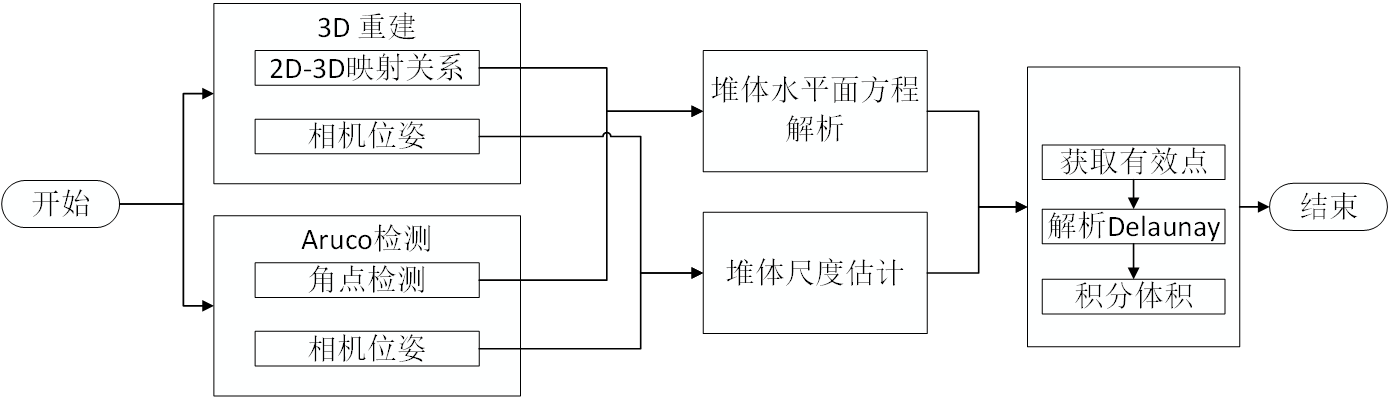
\includegraphics[height=5cm]{4GetV_pipeline.png}
    \caption{体积测算流程图}
    \label{fig:4GetV_pipeline}
  \end{figure}
\section{堆体水平面方程解析方法}
\label{sec:4.2}
\subsection{2D/3D点坐标检测}
\label{sec:4.2.1}
对于水平面的求解,其基本思路为求解落在堆体水平面上二维码的角点所在的坐标平面,或者求解已知角点和堆体水平面的实际空间位置关系,通过角点求解堆体实际水平面方程,二维码如图~\ref{fig:2VSLAM_Marker_detection}所示,将其作为媒介来估计平面方程。

首先检测2D点,可以利用二维码检测算法检测出场景中二维码的ID值,位置,大小,角点坐标等信息,检测结果如图~\ref{fig:4GetV_Marker_detection}所示。因为在场景中,二维码的布置都会有下侧两个角点直接落在水平面上,因此可以认为所有二维码的下侧角点所构成的平面即是场景的水平面。那么接下来即可将水平面的求解转化为二维码角点所在平面的求解。在检测的过程中,需要将所有2D图片的索引和角点的位置记录下即可。
\begin{figure}[H] % use float package if you want it here
  \centering
  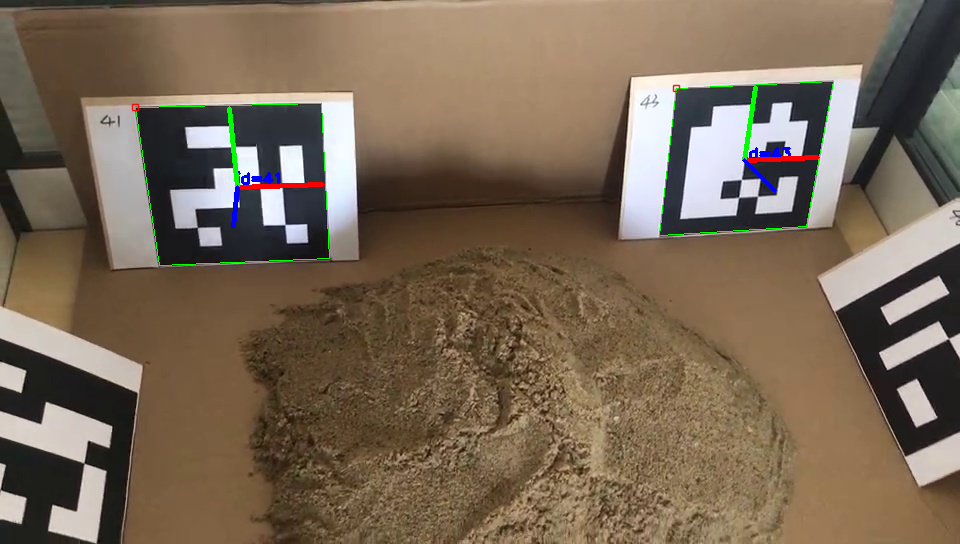
\includegraphics[height=8cm]{4GetV_Marker_detection.png}
  \caption{二维码检测示意图}
  \label{fig:4GetV_Marker_detection}
\end{figure}
其次再检测3D点,通过上述步骤,可以获得连续视频帧中每一帧的二维码角点的坐标值,同样的,可以直接将这些包含二维码的视频帧序列作为三维重建的输入以获取场景的点云,考虑到二维码角点被作为特征点时极易被检出,因此只需要通过稀疏点云,即可获取角点在二维图像中的坐标和三维重建点云中的三维坐标之间的对应关系。

在三维重建的过程中,可以获取到每一帧图像中所有特征点所对应的三维重建点云中的三维坐标,无论是稠密点云或者稀疏点云,都可以得到一个对应关系,但是考虑到遍历的效率问题,则选择稀疏点云中的点击作为遍历对象。在寻找对应关系的实际过程中,会遇到二维坐标无法映射到三维坐标点的情况,那么则会优先选择距离二维点坐标欧氏距离最近的点作为替代对象。此外,还需要注意的是,若所布置的二维码的所有下侧点都位于同一条直线上,那么这样就无法获取准确的水平面方程,因为经过同一直线的平面并不唯一,因此在布置坐标的过程中需要注意将所有二维码尽可能分散放置。
\subsection{平面方程优化方法}
\label{sec:4.2.2}
根据上述步骤,可以将待求的堆体水平面方程问题转化为求解N个三维点所在水平面方程的非线性优化问题。本文选择谷歌开源的Ceres solver库作为解决该非线性问题的工具,Ceres可以解决边界约束鲁棒非线性最小二乘法优化的问题,表达式如下:
\begin{equation}
\begin{array}{l}\underset x{min}\;\;\frac12\sum\rho_i(\parallel f_i(x_{i_1},...,x_{i_k})\parallel^2)
\\s.t.\;\;l_j\leq x_j\leq u_j\\\end{array}
\end{equation}
其中$\rho_i(\parallel f_i(x_{i_1},...,x_{i_k})\parallel^2$为残差块, $f_i(.)$为代价函数,代价函数的求解依赖于一系列参数$[x_{i_1},...,x_{i_k}]$所有参数构成参数块,限制边界分别为$l_j$,$u_j$。$\rho_i$为损失函数,其作用是减少异常值对优化结果的影响。
在利用Ceres解决非线性问题时,通常分为以下三个步骤:
1. 构建代价函数,也就是具体问题所对应的目标式,本小结具体解决N个三维点所在水平面的方程;

2. 通过代价函数构建待求解的优化问题;

3. 配置求解器参数并求解问题,在这一过程中主要是设定求解方程的方式。上述步骤如代码~\ref{code:chap3:get_plane}所示。
\begin{lstlisting}[
  language=C++,
  numbers=left,                
  numberstyle=\footnotesize,
  frame=single,     
  basicstyle=\small\tt,    
  escapeinside = '',
  caption={获取平面方程参数的~C++~实现},
  label={code:chap3:get_plane}]
  vector<vector<float>> plane_data1;
  vector<float> planex_data1 ,planey_data1, planez_data1;'//待优化量'
  '// 第一部分:构建代价函数模型'
  struct CURVE_FITTING_COST_plane
  {
    CURVE_FITTING_COST_plane (double x,double y,double z)
    :_x( x ), _y ( y ), _z ( z ) {}
    '// 残差的计算'
    template <typename T>
    bool operator() (
      const T* const plane,    
      T* residual ) const 
    {
      residual[0] = plane[0]*T(_x) + plane[1]*T(_y) 
                  + plane[2]*T(_z) + plane[3]; 
      return true;
    }
    const double _x, _y, _z;
  };

  int main ( int argc, char** argv )
  {   
    double plane[4] = {0.1,0.1,0.2,0};
    '// 第二部分:构建最小二乘问题'
    ceres::Problem problem2;
    for ( int i=0; i<planex_data1.size(); i++ ){
      problem2.AddResidualBlock 
      (new ceres::AutoDiffFunction<CURVE_FITTING_COST_plane,1,4> 
      (new CURVE_FITTING_COST_plane 
      (planex_data1[i], planey_data1[i],planez_data1[i])),
      nullptr,
      plane);
    }
    '// 第三部分:配置求解器'
    ceres::Solver::Options options2;    
    options2.linear_solver_type = ceres::DENSE_QR;
    options2.minimizer_progress_to_stdout = true; 
    ceres::Solver::Summary summary2;                 
    ceres::Solve ( options2, &problem2, &summary2 );
    for ( auto a:plane ) {
      outfile_kabc<<a*1/plane[3]<<endl;
      }
    return 0;
  }
\end{lstlisting}
对于任意平面方程,都可以利用以下方程通过确定4个参数的方式来确定唯一解析解。
\begin{equation}Ax+By+Cz+D= 0\label{equ:plane}\end{equation}
在迭代的过程中,同时需要确定每个带估计参数的初始值,最终可以得到方程的四个参数A,B,C,D。
\section{堆体尺度估计方法}
\label{sec:4.3}
由单目视觉重建出来的点云地图都存在没有确定尺度的问题,地图中的特征点坐标和相机的位姿都是相对尺度,即最常见的采取初始化成功后的前两帧作为单位尺度,后续的所有关键帧都以此为参考确定尺度。这样的做法可以获取到地图中所有描述的绝对尺度,但无法计算出实际尺度,本文提出两种结合二维码估计尺度大小的方法,通过在场景中引入已知尺度的二维码来确定所构点云地图的真实尺度,主要针对同一场景,计算两种SLAM的相机位姿或者两种SLAM中地图点坐标来确定相对尺度和绝对尺度之间的比例,从而确定绝对尺度。
\subsection{位姿法估计}
首先,获取绝对尺度的数据,由图~\ref{fig:getVolume_Aruco_detect}所示同时可以得到相机在某一个确定的二维码下的位姿,因为二维码自带确定的边长信息,因此可以得到带有绝对尺度的相机位姿($T_x$,$T_y$,$T_z$)。在实际的工程中需要注意,必须选择不同的相机对于同一二维码下的位姿,可以通过多帧图像序列获取到多个不同位姿。

其次,再获取同一批图像序列的相对尺度,通过三维重建的结果,就可以得到每一帧相机在参考坐标系下的位姿($T_x$,$T_y$,$T_z$),该位姿为相对尺度,因为只需要考虑到尺度的大小关系,因为不需要讨论不同坐标系之间的相对转化问题。

以上可以获取到多个针对同一场景的两种SLAM相机位姿估计结果,本文提出通过位姿来估计尺度的方法,因为两种SLAM方法估计出的相机位姿是基于不同的坐标系得到的,本文提出利用相机在不同坐标系下移动的欧式距离之间的比例来确定尺度,简化公式为:
\begin{equation}K\;=\;\frac{\triangle Pose_{rel}}{\triangle Pose_{abs}}  
\label{equ:getVolume_K}\end{equation}
同~\ref{sec:4.2.2}节,利用Ceres库得到最优解K值,计算如代码~\ref{code:chap3:get_k}所示:
\begin{lstlisting}[
  language=C++,
  numbers=left,                
  numberstyle=\footnotesize,
  frame=single,     
  basicstyle=\small\tt,    
  escapeinside = '',
  caption={获取尺度值的~C++~实现},
  label={code:chap3:get_k}]
  vector<vector<float>> colmap, opencv;
  vector<float> colmap_data1 ,opencv_data1;'//待优化量'
  '// 第一部分:构建代价函数模型'
  struct CURVE_FITTING_COST_k
  {
    CURVE_FITTING_COST_k (double x,double y)
    '// 残差的计算'
    template <typename T>
    bool operator() (
      const T* const k,     
      T* residual ) const     
    {
      residual[0] = T ( _y ) - ( k[0]*T ( _x ) ); // y-ax
      return true;
    }
    const double _x, _y;
  };
  int main ( int argc, char** argv )
  {   
    double k[1] = {0};
    '// 第二部分:构建最小二乘问题'
    ceres::Problem problem;
    for ( int i=0; i<colmap_data1.size(); i++ ){
      problem.AddResidualBlock 
      (new ceres::AutoDiffCostFunction<CURVE_FITTING_COST_k, 1, 1>
      (new CURVE_FITTING_COST_k 
      (opencv_data1[i], colmap_data1[i])),
      nullptr,
      k);
    }
    '// 第三部分:配置求解器'
    ceres::Solver::Options options;   
    options.linear_solver_type = ceres::DENSE_QR;  
    options.minimizer_progress_to_stdout = true;  
    ceres::Solver::Summary summary;              
    ceres::Solve ( options, &problem, &summary );  
    for ( auto a:k ) {
      outfile_kabc<<a<<endl;
      }
  return 0;
  }
\end{lstlisting}
只需要解出唯一参数K即可,在计算的过程中可以随机获取任意两帧之间的位姿,以减小误差。
\subsection{空间坐标点估计尺度}
对于尺度的估计,可以通过场景中已知点之间的距离通过投影获得点云之中点的实际坐标,但是空间中的已知点难以确定,而且也不易保持固定不变,符合以上规则的点的数量较少。因此考虑到场景中二维码标记的角点为研究对象,可以通过SLAM求得每一个二维码在图像中的位置以及四个角点的位置,因为角点极易识别,且任意两个角点之间的实际空间距离都能够简易测量得到。

通过第~\ref{cha:chap3}章三维重建的流程,可以获取到每一个点在二维图像中和三维空间点之间的对应关系,如图~\ref{fig:4GetV_sizebyPoint}所示表示的是同一个点在二维和三维之间的对应。因为图像中的任意两个二维码角点之间的距离都是已知的,那么也可以得到三维坐标中任意两个角点之间的绝对尺度,将这一尺度因子应用到整个地图中进行缩放,即可获得一个带有真实尺度的地图。
\begin{figure}[h] % use float package if you want it here
  \centering
  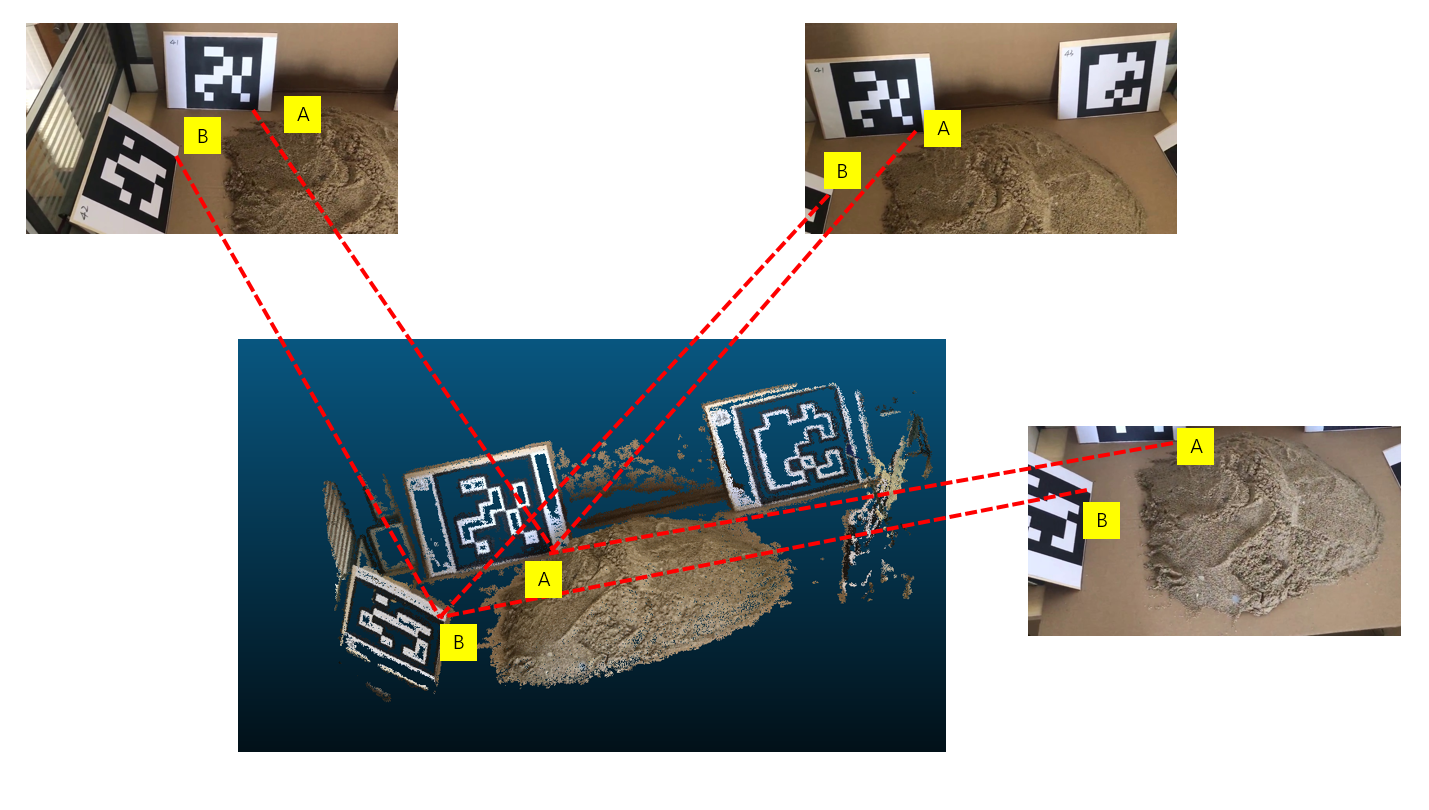
\includegraphics[height=6cm]{4GetV_sizebyPoint.png}
  \caption{根据空间点估计尺度流程图}
  \label{fig:4GetV_sizebyPoint}
\end{figure}
\section{堆体体积测量方法研究}
\label{sec:4.4}
根据以上两节可以获取三维重建后堆体点云的水平面方程和比例尺度,在此基础上可以进一步计算出堆体的实际体积,本文提出一种计算点云实际体积的方法,具体流程如下:

1. 将所有堆体点云中的3D点投影在水平面上,根据场景的实际空间约束和过滤方法提纯出有效3D点集;

2. 通过空间变换,将三维空间点转化为水平面上的点2D点集;

3. 对所有2D点集求Delauncy三角形,计算每个三角形对应的水平高度,得到三棱柱体积;

4. 剔除异常三棱柱,将所有有效的三棱柱积分求和得到总体积。

流程图如图~\ref{fig:4GetV_volume}所示。
\begin{figure}[h] % use float package if you want it here
  \centering
  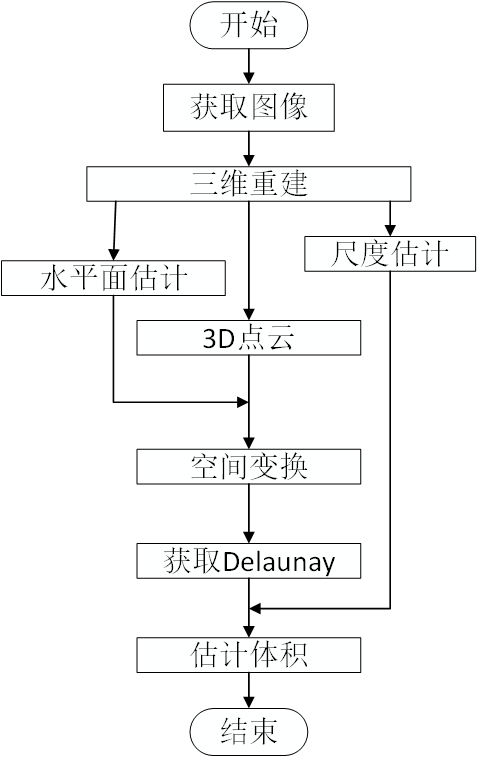
\includegraphics[height=10cm]{4GetV_volume.png}
  \caption{纯视觉测量体积流程图}
  \label{fig:4GetV_volume}
\end{figure}
\subsection{有效3D点集获取}
\label{sec:4.4.1}
通过第~\ref{cha:chap3}章的方法,可以对堆体场景获取三维稀疏点云和稠密点云,在生成点云的过程中会把部分非感兴趣区域的内容和一些离散的误差噪音点添加至点云结果中。针对这两种情况,本文分别提出以下对应的解决方法:

1. 针对非感兴趣区域,本文通过三维空间平面方程对非感兴趣区域直接进行切割剔除;

2. 针对随机误差噪音点,本文通过离群点检测算法进行剔除。

对于方案1,对于重建后的三维点云,只需要收集感兴趣区域内的3D点集,如图~\ref{fig:4GetV_interesting}所示,只有红色框图内区域是体积测量的感兴趣区域,通过上一节求出的水平面方程和二维码的底边点坐标共同约束求出空间切面方程对场景进行切割。
\begin{figure}[H] % use float package if you want it here
  \centering
  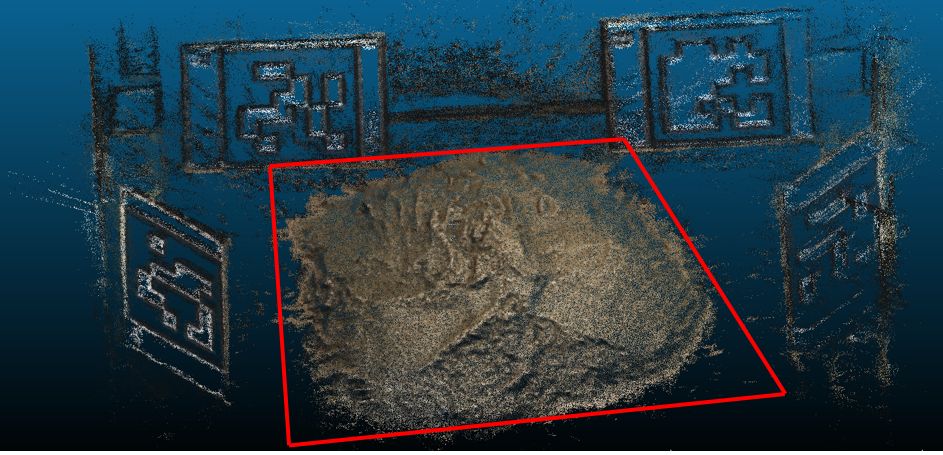
\includegraphics[height=4.5cm]{4GetV_interesting.png}
  \caption{三维重建感兴趣区域示意图}
  \label{fig:4GetV_interesting}
\end{figure}
对于方案2,本文采用统计滤波器即为对每个点的邻域进行一个统计分析,并修剪掉一些不符合标准的点,具体方法为在输入数据中对点到临近点的距离分布的计算,对每一个点,计算它到所有临近点的平均距离(假设得到的结果是一个高斯分布,其形状是由均值和标准差决定),那么平均距离在标准范围之外的点,可以被定义为离群点并从数据中去除。采用统计滤波对点云中的离散点进行滤波对比如图~\ref{fig:4GetV_3dconstr_filter}所示。
\begin{figure}[H]
  \centering
    \subcaptionbox{对点云统计滤波前}{\label{fig:4GetV_3dconstr_noise}
    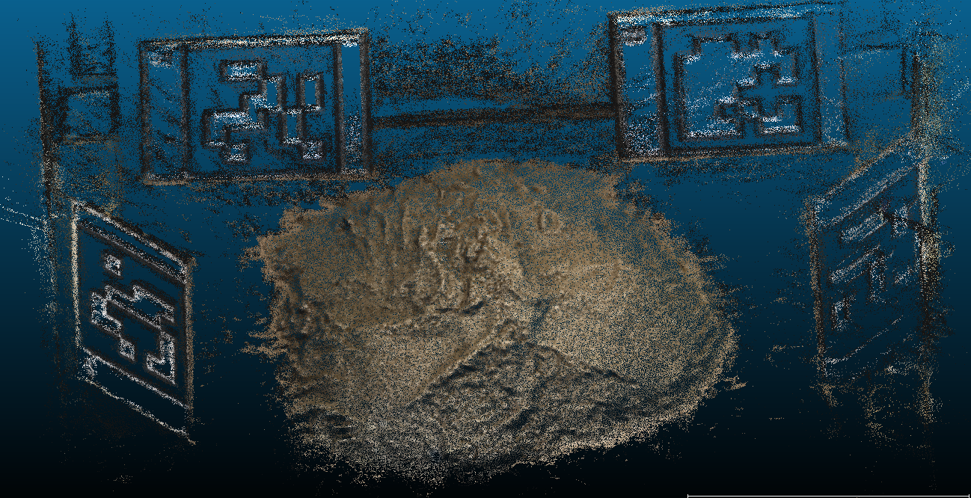
\includegraphics[width=8cm]{4GetV_3dconstr_noise.png}}
  \vskip0.5cm
    \subcaptionbox{对点云统计滤波后}{\label{fig:chap1:4GetV_3dconstr_nonoise}
 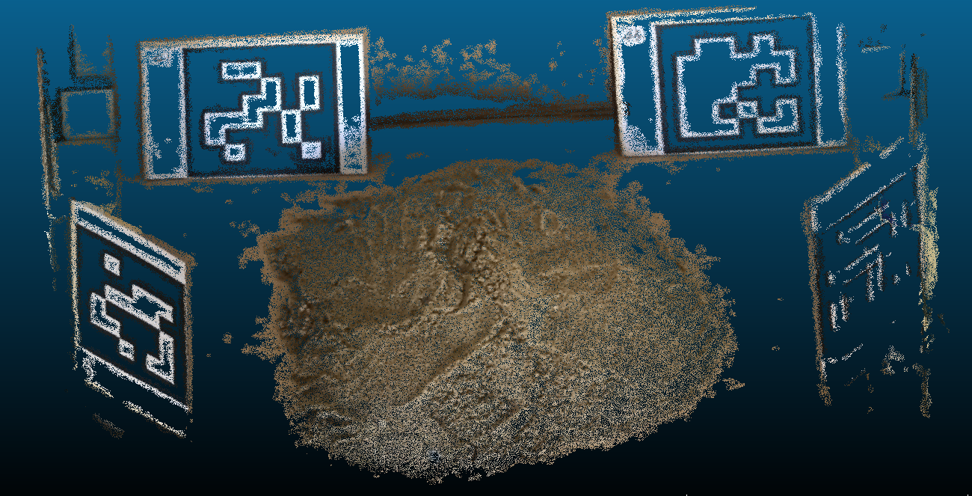
\includegraphics[width=8cm]{4GetV_3dconstr_nonoise.png}}
  \caption{点云统计滤波前后效果对比示意图}\label{fig:4GetV_3dconstr_noise}
\end{figure}
通过以上步骤,可以求出有关堆体的有效3D点集,接下来需要将所有三维点云投影至二维平面上获取2D点集,简略步骤如下:
1. 通过~\ref{sec:4.2}节获取点云水平面和参考坐标系中的xy平面方程的法向量分别为U(A,B,C)和V(0,0,1);

2. 将所有的3D点集O($x_o$,$y_o$,$z_o$)根据以下公式投影水平面上,获取新的3D点集P($x_p$,$y_p$,$z_p$);
\begin{equation}
  \begin{split}
  x_p=\frac{(B^2+C^2)x_o-A(By_o+Cz_o+D)}{A^2+B^2+C^2}\\
  y_p=\frac{(A^2+C^2)y_o-B(Ax_o+Cz_o+D)}{A^2+B^2+C^2}\\
  z_p=\frac{(A^2+B^2)z_o-C(Ax_o+By_o+D)}{A^2+B^2+C^2}
  \label{equ:pxyz}
  \end{split}
\end{equation}
同时也可以根据公式计算出每一个三维空间点到水平面的方程的距离
\begin{equation}
d\;=\frac{\left|Ax_0+By_0+Cz_0+D\right|}{\sqrt{A^2+B^2+C^2}}
\end{equation}

3. 计算旋转角度:
\begin{equation}
\theta=arc\cos(\frac{U\cdot V}{\left|U\right|\left|V\right|})
\end{equation}

4. 计算旋转轴:在计算旋转角时可知,旋转角所在的平面为有P和Q所构成的平面,那么旋转轴必垂直该平面。
假定旋转前向量为a($a_1$, $a_2$, $a_3$), 旋转后向量为b($b_1$, $b_2$, $b_3$)。由叉乘定义得旋转轴k($k_1$, $k_2$, $k_3$)为
\begin{equation}
\begin{pmatrix}c_1\\c_2\\c_3\end{pmatrix}=\begin{pmatrix}a_2b_3-a_3b_2\\a_3b_1-a_1b_3\\a_1b_2-a_2b_1\end{pmatrix}
\end{equation}

5. 根据罗德里格旋转公式将旋转角,旋转轴的表达转化为旋转矩阵R
\begin{equation}R=\cos \theta I+(1-\cos \theta) k k^{\top}+\sin \theta k^{\wedge}\end{equation}

6. 将3D点集P($x_p$,$y_p$,$z_p$)右乘上述旋转矩阵R可以得到一系列在同一平面上(所有转变后的点z值都相同)的3D点集,提取所有3D点的x,y值构成2D点集p($x$,$y$)。
\subsection{Delaunay三角网}
\label{sec:4.4.3}
通过~\ref{sec:4.2}小结,可以得到在由在同一平面上的3D点集转化成的2D点集和每一个2D点集对应的距离值d。在本节中将对2D点集进行三角剖分,获得Dealunay三角网,Delaunay三角网是一系列相连的但不重叠的三角形的集合, 而且这些三角形的外接圆不包含这个面域的其他任何点,如图~\ref{fig:4GetV_Delaunay}所示。
\begin{figure}[H] % use float package if you want it here
  \centering
  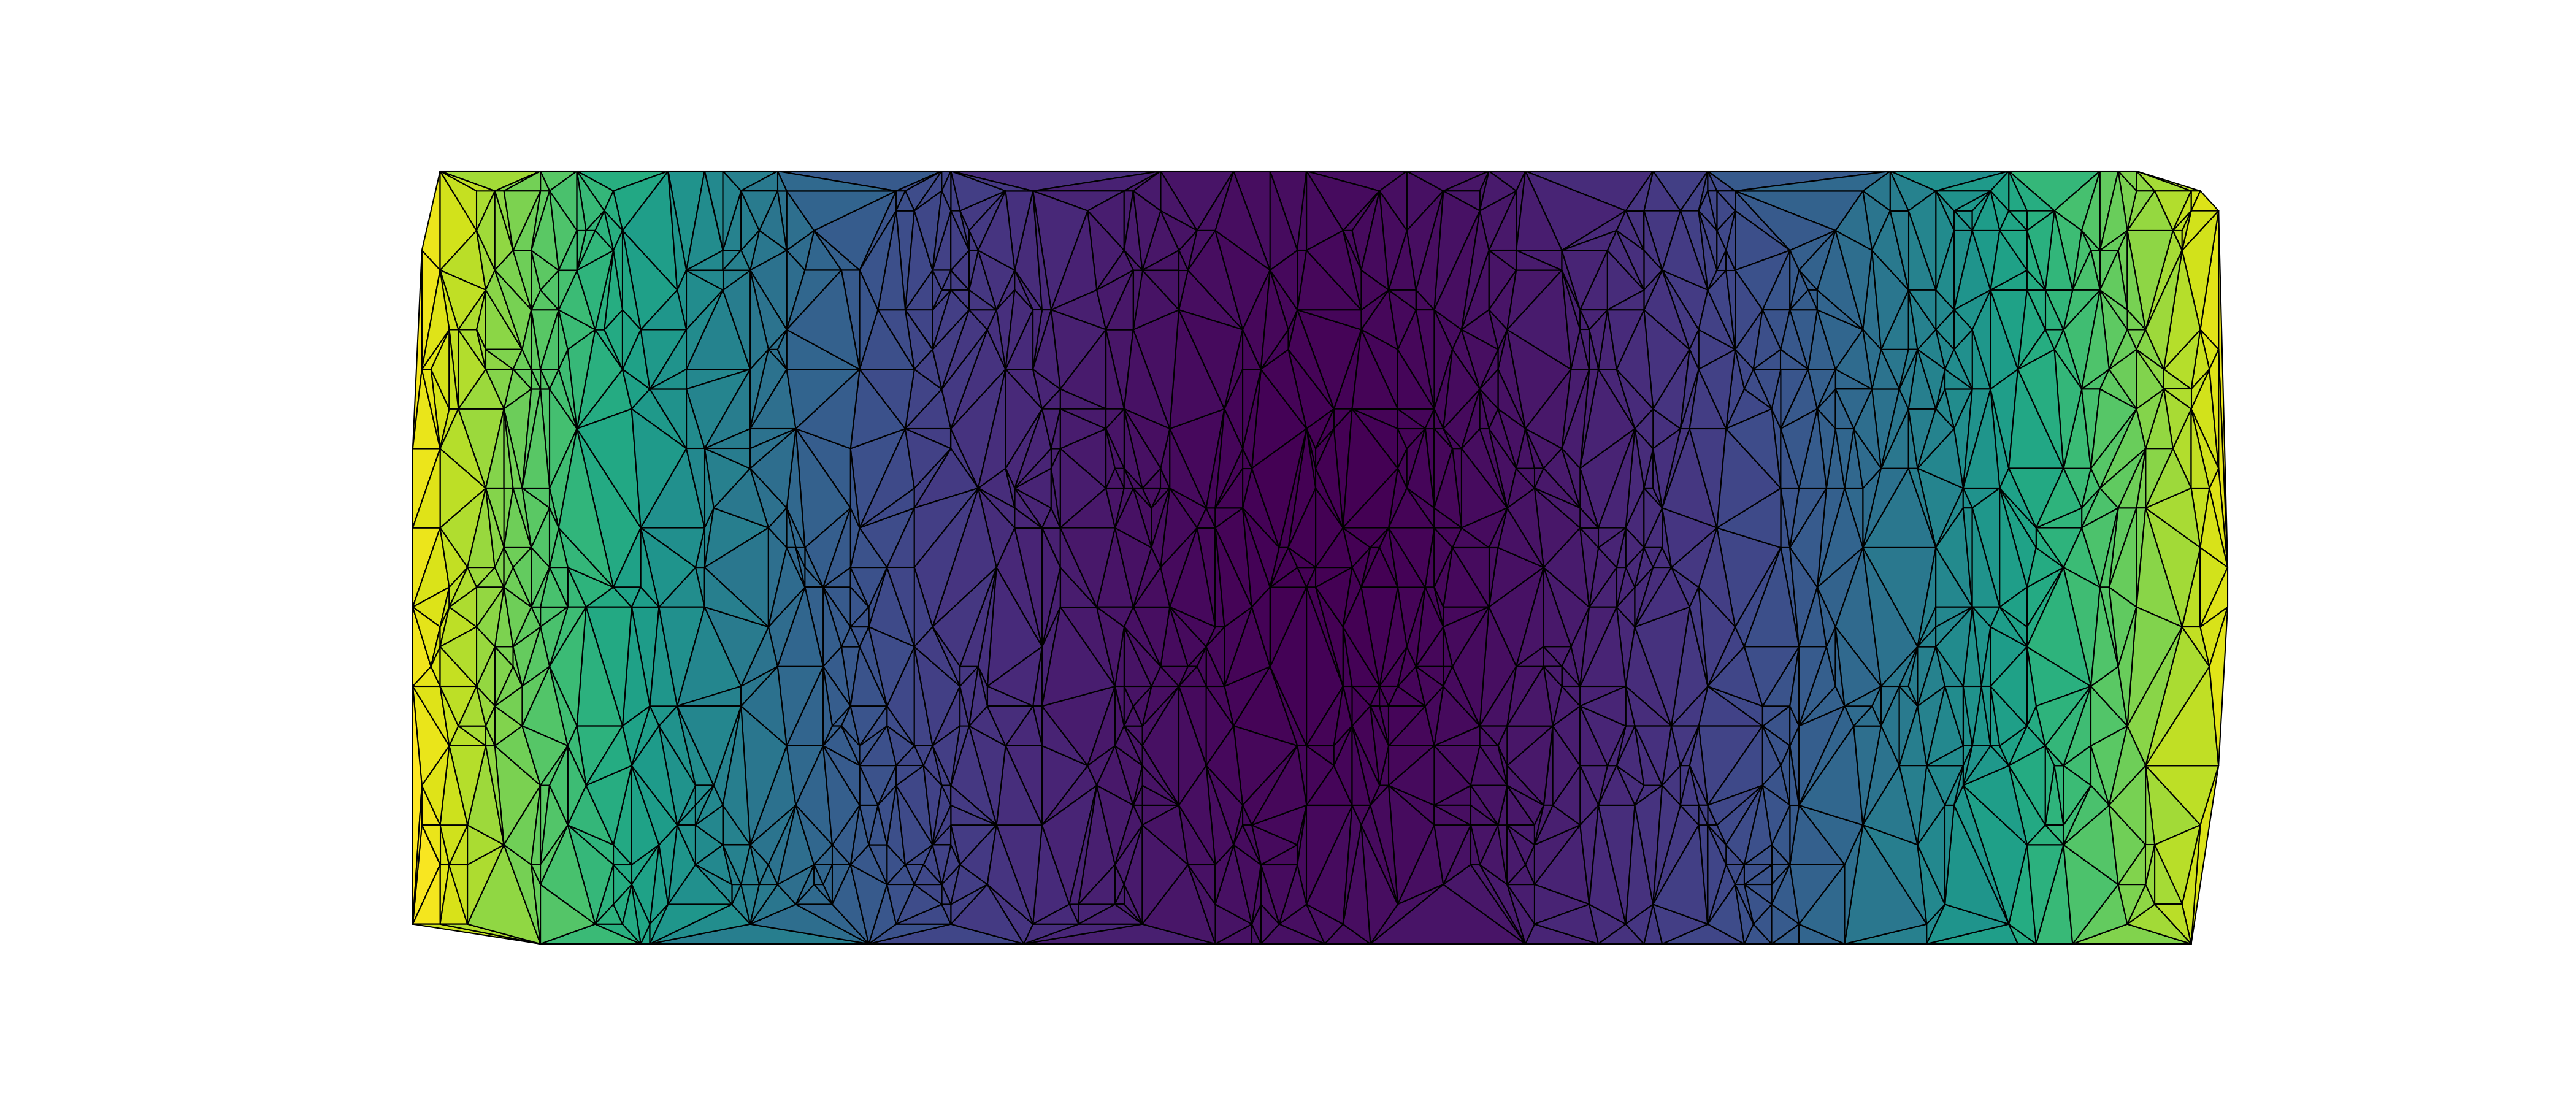
\includegraphics[height=6cm]{4GetV_Delaunay.png}
  \caption{Delaunay三角网示意图}
  \label{fig:4GetV_Delaunay}
\end{figure}
获取Delaunay三角网格的一般步骤为: 

1. 构造一个超级三角形,包含所有散点,放入三角形链表;

2. 将点集中的散点依次插入,在三角形链表中找出其外接圆包含插入点的三角形(称为该点的影响三角形),删除影响三角形的公共边,将插入点同影响三角形的全部顶点连接起来,从而完成一个点在Delaunay三角形链表中的插入;

3. 根据优化准则对局部新形成的三角形进行优化。将形成的三角形放入Delaunay三角形链表;

4. 循环执行上述第2步,直到所有散点插入完毕。\\
由于Delaunay剖分具备最接近性和区域性的特性,可以对点集所构成的平面进行拟合。通过以上流程可以获得三角形集合以及三角形中每个顶点对应的距离,取三个顶点距离的平均值作为三棱柱的高,即可获得所有三棱柱的体积。
\subsection{积分三棱柱}
\label{sec:4.4.4}
通过以上步骤,可以将三维重建后点云体积的求解转化成对多个三棱柱积分的求解,因为所有三棱柱的体积值都分布在某一个区间内(并不完全服从正太分布),对于部分偏差较大的三棱柱体积值应该通过算法进行剔除。本文采用箱形图的方法来处理这一问题,箱形图不受异常值的影响,能够准确稳定地描绘出数据的离散分布情况,同时也利于数据的清洗,箱形图如图~\ref{fig:4GetV_boxplot}所示。
\begin{figure}[t] % use float package if you want it here
  \centering
  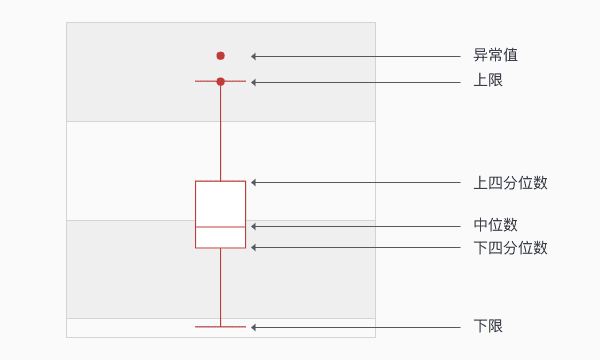
\includegraphics[height=6cm]{4GetV_boxplot.png}
  \caption{箱形图示意图}
  \label{fig:4GetV_boxplot}
\end{figure}
主要需要求解出数据中的5个特征数据值,包括下四分位数Q1,上四分位数Q3,四分位距IQR=Q3-Q1,以及上限Q3+1.5IQR和下限Q1-1.5IQR,对于上下限之外的内容需要剔除,最终结合\label{sec:4.3}估算出的尺度,以及所有有效三棱柱的体积按照公式~\ref{equ:get_volume}即可估计出物体中感兴趣区域的实际体积值。
\begin{equation}
  V\;=K^3\;\ast\sum_i\frac13\ast S_\bigtriangleup\times\sum_{j=1}^3d_j\label{equ:get_volume}
\end{equation}
\section{本章小结}
本章提出了一种面向堆体场景的体积测量方法,主要包括水平面方程的求解,尺度值的估计以及计算3D点云体积等流程,该方法完全基于纯视觉方式实现,在获取到堆体三维点云后,可以自动化估计出堆体的整体体积。

本章重点分析了堆体体积测量的可行性和数学描述过程,包含通过位姿法或者空间点坐标值法,利用非线性优化估计出堆体场景实际尺度和堆体点云相对尺度之间的比例关系;通过2D角点获取对应3D映射点,将水平面方程求解转化求解点集共面方程的问题;最后结合尺度估计值和水平面投影以及空间坐标变换求解Delaunay三角形,积分三棱柱以估计出堆体点云的实际体积。

本章以无人机的自主定位和飞行和高精度的三维重建为基础,提出了面对堆体场景的纯视觉体积测量技术,完整流程可以自动化完成,复用于相似场景。






